\documentclass{article}
\usepackage[spanish,es-nodecimaldot]{babel}
\usepackage[utf8]{inputenc}
\usepackage[letterpaper,top=2.2cm,bottom=2.5cm,left=2.5cm,right=2.5cm,headheight=70pt]{geometry}

% Paquetes matemáticos y visuales
\usepackage{amsmath}
\usepackage{amssymb}
\usepackage{graphicx}
\graphicspath{{imagenes/}{../imagenes/}}
\usepackage[colorlinks=true, allcolors=blue, hypertexnames=false]{hyperref}
\usepackage{fancyhdr}
\usepackage{multicol}
\usepackage{float}
\usepackage{listings}
\usepackage{xcolor}
\usepackage{array}
\usepackage{longtable}
\usepackage{booktabs}
\usepackage{tabularx}

% Configuración de listados de código con soporte de caracteres en español
\lstset{
    basicstyle=\ttfamily\scriptsize,
    breaklines=true,
    frame=single,
    backgroundcolor=\color{gray!8},
    keywordstyle=\color{blue}\bfseries,
    commentstyle=\color{green!50!black}\itshape,
    stringstyle=\color{red!70!black},
    numbers=left,
    numberstyle=\tiny\color{gray},
    numbersep=5pt,
    tabsize=4,
    showspaces=false,
    showstringspaces=false,
    literate=
        {á}{{\'a}}1 {é}{{\'e}}1 {í}{{\'i}}1 {ó}{{\'o}}1 {ú}{{\'u}}1
        {Á}{{\'A}}1 {É}{{\'E}}1 {Í}{{\'I}}1 {Ó}{{\'O}}1 {Ú}{{\'U}}1
        {ñ}{{\~n}}1 {Ñ}{{\~N}}1 {¿}{{?`}}1 {¡}{{!`}}1
}

\pagestyle{fancy}
\fancyhf{}
\setlength{\headheight}{70pt}

% Encabezado UTA / FISEI
\fancyhead[C]{%
    \begin{minipage}[c]{2.5cm}
        \centering
        
\includegraphics[width=2.2cm]{imagenes/uta.png}
    \end{minipage}%
    \hfill
    \begin{minipage}[c]{10cm}
        \centering
        \small \textbf{UNIVERSIDAD TÉCNICA DE AMBATO} \\[0.1cm]
        \scriptsize \textit{FACULTAD DE INGENIERÍA EN SISTEMAS ELECTRÓNICA E INDUSTRIAL} \\[0.1cm]
        \scriptsize \textbf{CARRERA DE SOFTWARE} \\[0.1cm]
        \scriptsize \textbf{CICLO ACADÉMICO: JULIO -- DICIEMBRE 2026}
    \end{minipage}%
    \hfill
    \begin{minipage}[c]{2.5cm}
        \centering
        
\includegraphics[width=2.2cm]{imagenes/fisei.png}
    \end{minipage}%
}
\fancyfoot[C]{\thepage}

\begin{document}

\begin{center}
    {\Large \textbf{INFORME DE GUÍA PRÁCTICA -- TALLER DE ACS}} \\[0.2cm]
    {\large \textbf{EVALUACIÓN DEL ASEGURAMIENTO DE LA CALIDAD DEL SOFTWARE (ACS) EN TECHSTORE (POST-MEJORA)}}
\end{center}

\vspace{0.2cm}

\section{Portada}
\begin{flushleft}
\renewcommand{\arraystretch}{1.2}
\begin{tabular}{ p{5.5cm} p{10cm} }
    \textbf{Tema:} & Evaluación del Aseguramiento de la Calidad del Software (ACS) en TechStore (Post-Mejora) \\
    \textbf{Unidad de Organización Curricular:} & PROFESIONAL. \\
    \textbf{Nivel y Paralelo:} & Séptimo - A \\
    \textbf{Alumnos participantes:} & Tasinchano Tite Audi Alexander \\
                                   & Hurtado Cristian \\
    \textbf{Asignatura:} & GESTIÓN DE CALIDAD DEL SOFTWARE \\
    \textbf{Docente evaluador:} & Ing. Mg. Alex Maigua Quinteros \\
    \textbf{Fecha de entrega:} & 16 de Octubre de 2026 \\
\end{tabular}
\end{flushleft}

\vspace{0.3cm}

\section{Informe de guía práctica}

\subsection{Objetivos}
\subsubsection{Objetivo general}
Evaluar integralmente la calidad del sistema empresarial TechStore sobre el ERP Odoo 16 tras las remediaciones técnicas implementadas en el taller anterior, aplicando los principios, marcos y elementos estructurales del Aseguramiento de la Calidad del Software (ACS / SQA) bajo las directrices de los estándares ISO/IEC 12207, ISO/IEC 25010 y el modelo CMMI v2.0, mediante la auditoría de elementos formales, la comprobación de tareas ejecutadas, la formulación de metas cuantitativas y el cálculo analítico de métricas de rendimiento y tasa de error frente a la línea base previa.

\subsubsection{Objetivos específicos}
\begin{itemize}
    \item Evaluar el grado de existencia y formalidad de los siete componentes esenciales del Aseguramiento de Calidad del Software (Políticas, Estándares, Procesos, Roles, Pruebas, Métricas y Evidencias) en el módulo TechStore post-mejora, formulando propuestas de evidencias concretas y verificables para aquellos elementos no formalizados.
    \item Identificar y catalogar con base en el código fuente las tareas del ACS que ya se encuentran activamente operativas en el sistema ERP, asociando validaciones de entrada, control preventivo de errores, verificación unitaria y monitoreo transaccional con sus artefactos de software correspondientes.
    \item Definir un conjunto de al menos cinco metas cuantitativas, medibles y viables de ACS, fundamentadas en el comportamiento observado tras la corrección de fórmulas matemáticas, la erradicación de retardos bloqueantes y la incorporación de restricciones de integridad.
    \item Medir de manera cuantitativa los tiempos de respuesta de las APIs CRUD de clientes, productos y ventas en la versión post-mejora, calculando analíticamente la tasa de error residual y el tiempo promedio transaccional para contrastarlos con los datos históricos de las 9 pruebas de la línea base previa.
    \item Emitir un dictamen técnico crítico sobre el estado actual de calidad del sistema, detallando las falencias estructurales que aún persisten en la dimensión del proceso y delineando un plan de mejora continua para iteraciones futuras.
\end{itemize}

\subsection{Modalidad}
Presencial y trabajo colaborativo de desarrollo en laboratorio de software.

\subsection{Tiempo de duración}
\begin{itemize}
    \item Horas presenciales: 4
    \item Horas no presenciales: 2
\end{itemize}

\subsection{Instrucciones}
Las actividades se desarrollan sobre el repositorio del sistema TechStore implementado como módulo personalizado en la plataforma Odoo 16 Community desplegada mediante Docker y PostgreSQL:
\begin{enumerate}
    \item Realizar una inspección exhaustiva de las modificaciones introducidas en el taller anterior sobre los modelos de datos (\texttt{techstore.customer}, \texttt{techstore.product}, \texttt{techstore.sale.order}).
    \item Auditar el cumplimiento de los componentes de gobernanza de calidad del software (Políticas, Estándares, Procesos, Roles, Pruebas, Métricas y Evidencias).
    \item Identificar en el repositorio existente las tareas de control y aseguramiento que ya están ejecutándose activamente, absteniéndose de inventar tareas no existentes.
    \item Formular metas cuantitativas de calidad con umbrales de aceptación derivados de la evidencia empírica.
    \item Ejecutar y tabular mediciones de tiempo de respuesta de los endpoints CRUD de la API REST, determinando la tasa de error y el tiempo promedio de respuesta para comparar con el estado inicial.
    \item Redactar el análisis crítico final respondiendo con fundamentación técnica y metodológica las tres interrogantes de evaluación de calidad.
\end{enumerate}

\textbf{Listado de equipos y materiales generales empleados en la guía práctica:}
\begin{itemize}
    \item Computador de desarrollo x86\_64 (Intel Core i7, 16 GB de memoria RAM, almacenamiento SSD NVMe).
    \item Sistema operativo Linux (kernel 6.x) con entorno de terminal Bash.
    \item Motor de contenedores Docker Engine v24+ y Docker Compose v2+.
    \item Plataforma ERP Odoo 16.0 Community Edition y Servidor de Base de Datos PostgreSQL 15.
    \item Entornos de desarrollo: Visual Studio Code, Antigravity IDE, Python 3.10/3.14 con bibliotecas \texttt{requests}, \texttt{matplotlib}, \texttt{pytest}.
    \item Compilador tipográfico \texttt{pdflatex} y \texttt{bibtex}.
\end{itemize}

\textbf{TAC (Tecnologías para el Aprendizaje y Conocimiento) empleados en la guía práctica:}
\begin{itemize}
    \item[$\boxtimes$] Inteligencia Artificial generativa y analítica como asistente de revisión y verificación de calidad.
    \item[$\boxtimes$] Plataformas educativas institucionales y entornos virtuales de aprendizaje (Moodle UTA).
    \item[$\boxtimes$] Controladores de versiones distribuidos (Git / GitHub) para trazabilidad de cambios.
\end{itemize}

\subsection{Actividades por desarrollar}
\begin{enumerate}
    \item Diagnóstico del Aseguramiento de Calidad del Software (ACS) en TechStore tras las mejoras funcionales y no funcionales aplicadas.
    \item Elaboración de la matriz de evaluación de los siete elementos esenciales de ACS con propuestas de evidencias para los faltantes.
    \item Catalogación estructurada de las tareas de ACS que ya operan dentro del código del sistema.
    \item Definición de metas cuantitativas de calidad basadas en la evidencia experimental.
    \item Toma de tiempos de respuesta de las APIs CRUD (clientes, productos y órdenes de venta), cálculo formal de tasa de error y tiempo promedio comparado frente al taller previo.
    \item Discusión crítica sobre la calidad del software, elementos pendientes de implementación y recomendaciones de ingeniería a futuro.
\end{enumerate}

\newpage

\subsection{Desarrollo}

\subsubsection{Contexto y Antecedentes de la Refactorización de TechStore}
En el taller previo, el sistema TechStore (módulo de gestión comercial y ventas montado sobre Odoo 16) presentaba severas falencias en su línea base que comprometían críticamente tanto la integridad contable como la estabilidad de la infraestructura:
\begin{enumerate}
    \item \textbf{Cálculos aritméticos y fiscales erróneos:} El método \texttt{\_compute\_subtotal} sumaba la cantidad y el precio unitario en lugar de multiplicarlos (\texttt{cantidad + precio\_unitario - descuento}), aplicaba una alícuota distorsionada de IVA del 5\% en contraposición a la tasa tributaria legal del 15\% vigente en el Ecuador según el Servicio de Rentas Internas (SRI), y alteraba arbitrariamente los precios duplicándolos si la cantidad superaba las 5 unidades.
    \item \textbf{Inexistencia de validaciones de integridad de datos:} No existían restricciones contra clientes duplicados con igual número de identificación o correo electrónico, se permitía registrar productos con costos o existencias negativas, y se admitían órdenes de venta con cantidades nulas o desproporcionadas respecto al inventario en bodega.
    \item \textbf{Degradación deliberada de rendimiento transaccional:} El método \texttt{create} introducía pausas bloqueantes con \texttt{time.sleep(0.10)} y latencias artificiales de hasta 3.5 segundos, colapsando los hilos del servidor ante solicitudes concurrentes.
    \item \textbf{Carencia absoluta de pruebas y métricas:} No se contaba con una batería de pruebas automatizadas documentadas ni con indicadores que cuantificaran la estabilidad o el desempeño del software.
\end{enumerate}

En la fase de refactorización previa se corrigieron las fórmulas matemáticas fijando el cálculo exacto de subtotal ($Subtotal = Cantidad \times Precio - Descuento$), el IVA legal al 15\% (\texttt{TASA\_IVA = 0.15}) con redondeo comercial consistente, se eliminaron los bloqueos artificiales, y se agregaron validaciones mediante restricciones de base de datos (\texttt{\_sql\_constraints}) y restricciones de modelo (\texttt{@api.constrains}). El presente trabajo evalúa este sistema post-mejora desde la óptica metodológica del Aseguramiento de la Calidad del Software (ACS / SQA) \cite{pressman2014, sommerville2011}.

\begin{figure}[H]
    \centering
    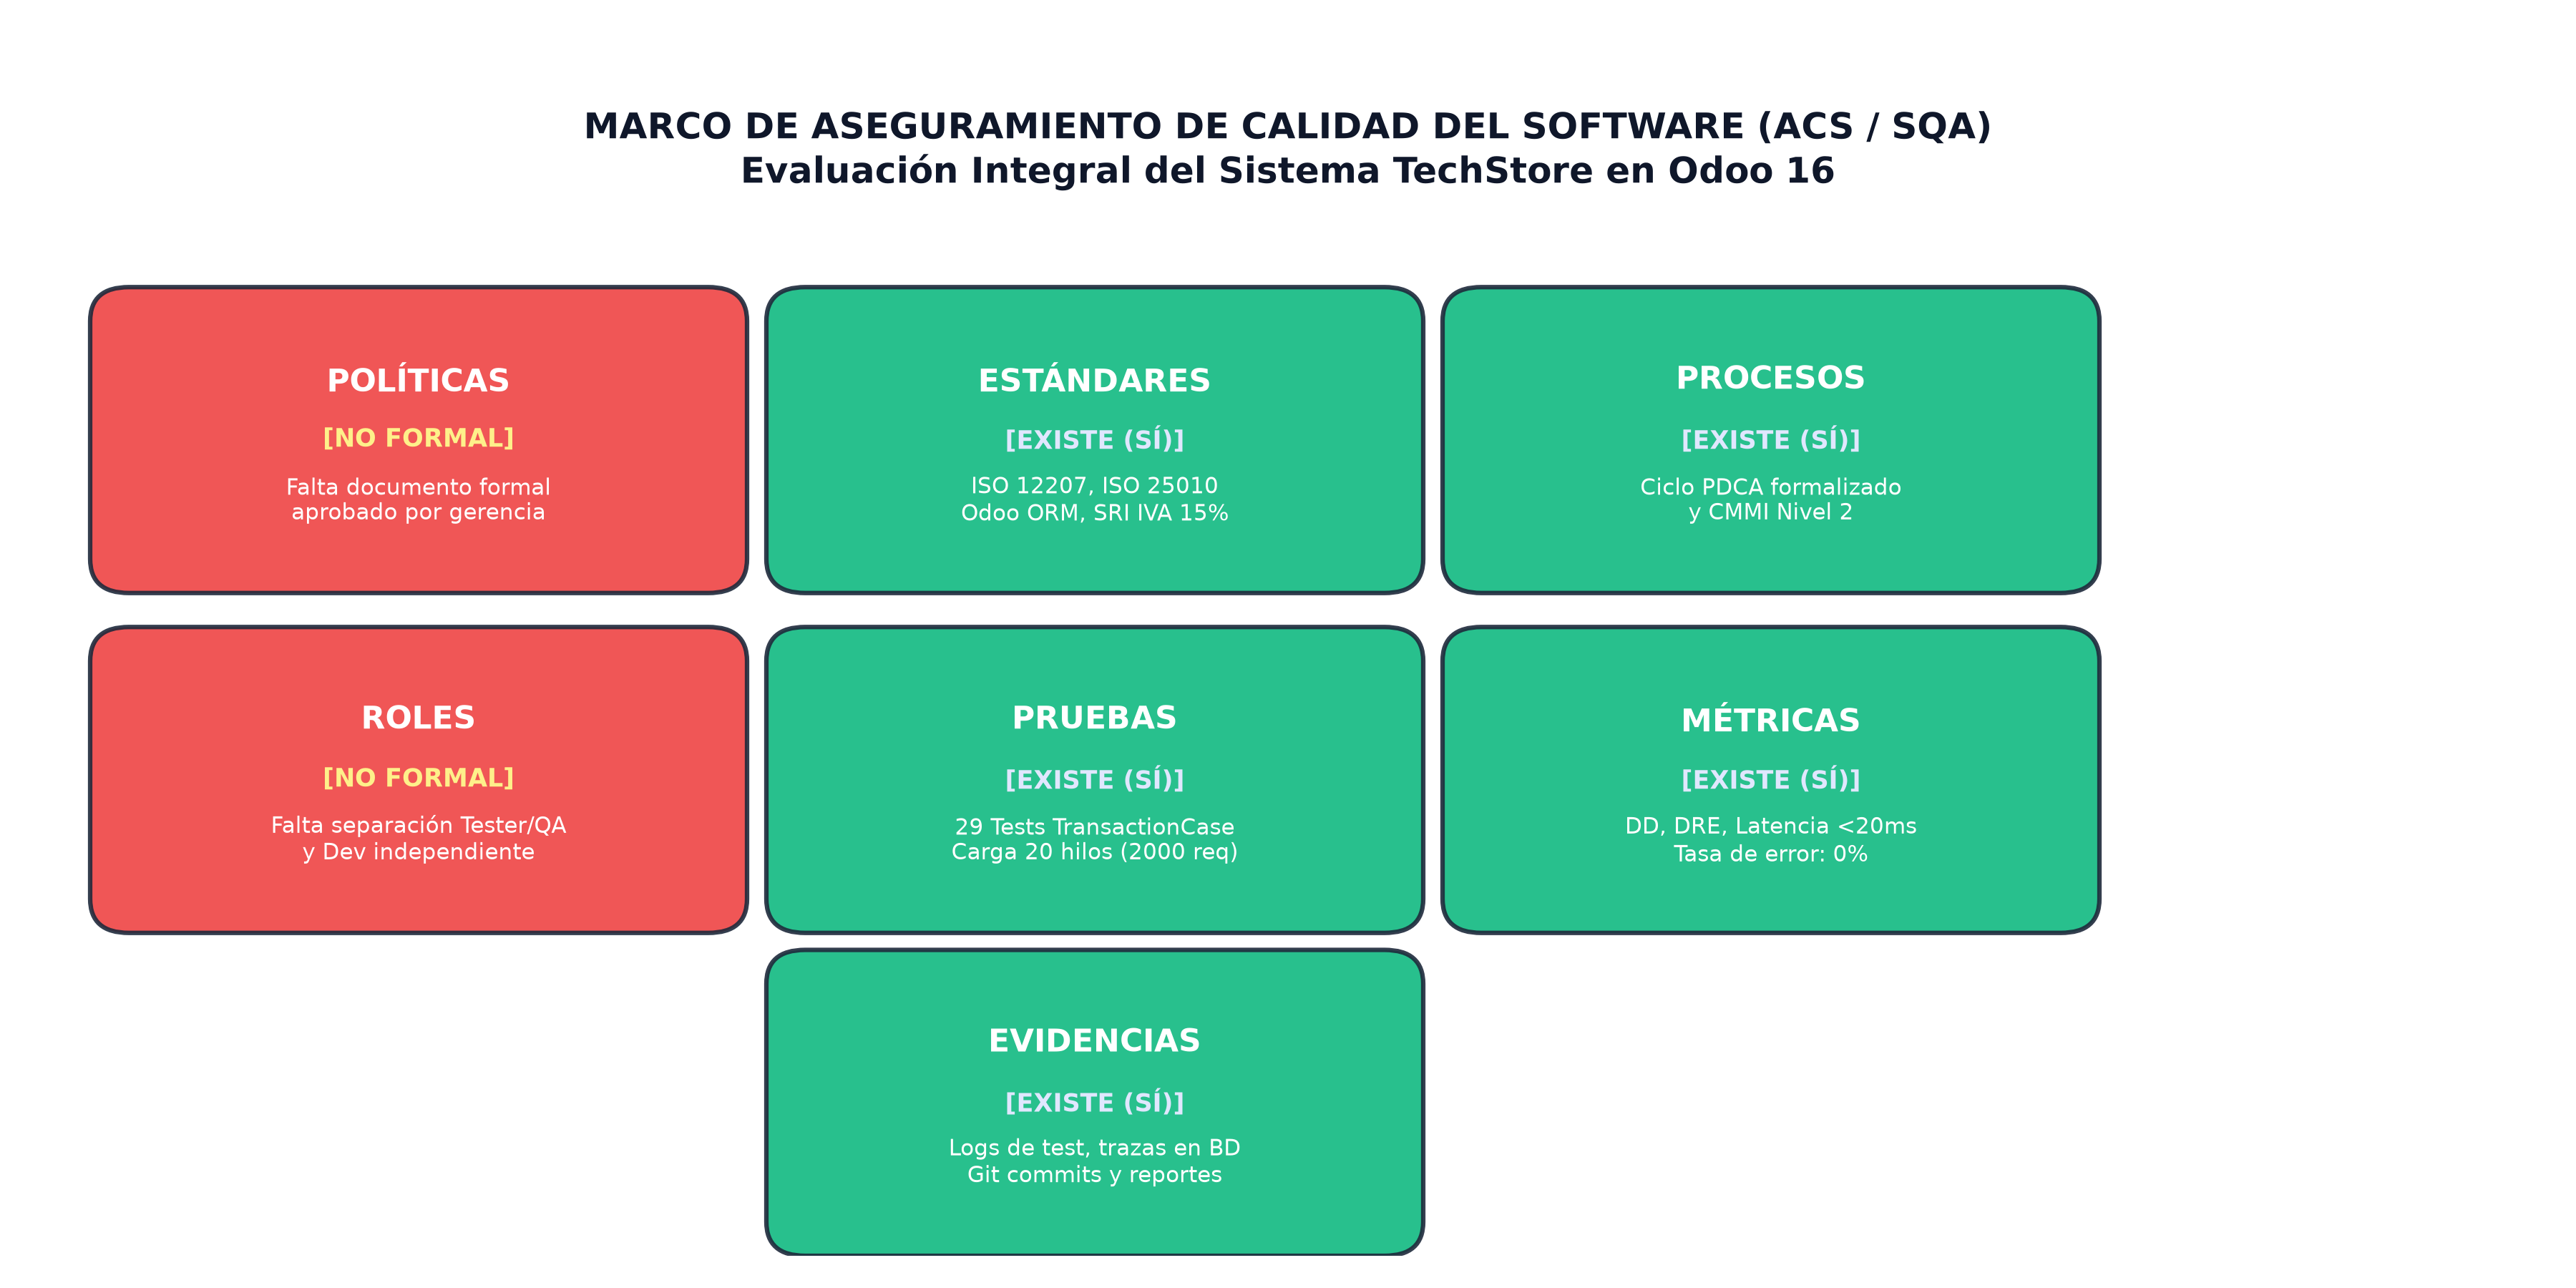
\includegraphics[width=0.92\textwidth]{imagenes/elementos_acs_techstore.png}
    \caption{Marco de Aseguramiento de la Calidad del Software (ACS) y evaluación de componentes en TechStore.}
    \label{fig:elementos_acs}
\end{figure}

\clearpage

\subsubsection{Evaluación de Elementos del ACS en TechStore (Post-Mejora)}
El Aseguramiento de la Calidad del Software (ACS o SQA) es un patrón de actividades planificadas y sistemáticas necesarias para proveer la confianza adecuada de que el producto satisfará los requisitos técnicos y normativos del cliente \cite{pressman2014}. En el Cuadro \ref{tab:evaluacion_acs} se auditan los siete elementos estructurales del ACS en TechStore:

\begin{table}[H]
\centering
\small
\caption{Evaluación de Elementos del Aseguramiento de Calidad del Software (ACS) en TechStore.}
\label{tab:evaluacion_acs}
\renewcommand{\arraystretch}{1.25}
\begin{tabularx}{\textwidth}{p{2.6cm}cp{10.2cm}}
\toprule
\textbf{Elemento ACS} & \textbf{¿Existe?} & \textbf{¿Cómo se evidencia? / Propuesta de evidencia si no existe} \\
\midrule
\textbf{Políticas} & \textbf{No} & 
\textbf{Propuesta de evidencia:} Formulación y aprobación por parte de la Dirección de Tecnología de un \textit{Manual de Políticas de Calidad del Software de TechStore}, donde se estipule como regla corporativa obligatoria: (1) Tolerancia cero a errores en fórmulas contables e impositivas (IVA al 15\%); (2) Prohibición estricta de desplegar cambios a producción que no superen el 100\% de las pruebas unitarias; y (3) Política de control riguroso de inventarios impidiendo en todo nivel saldos negativos. \\
\midrule
\textbf{Estándares} & \textbf{Sí} & 
\textbf{Evidencia en el sistema:} Se evidencia en la adopción explícita de marcos internacionales: (1) \textbf{ISO/IEC 12207} \cite{iso12207} para la estructuración de las fases del ciclo de vida del software (análisis, diseño, desarrollo, pruebas); (2) \textbf{ISO/IEC 25010} \cite{iso25010} para la evaluación de adecuación funcional, fiabilidad y eficiencia; (3) Convenciones y estándares de codificación oficiales de Odoo ORM (uso de \texttt{\_sql\_constraints}, decoradores \texttt{@api.constrains}, \texttt{@api.depends}); y (4) Marco legal tributario ecuatoriano del SRI para el cálculo impositivo. \\
\midrule
\textbf{Procesos} & \textbf{Sí} & 
\textbf{Evidencia en el sistema:} Se evidencia mediante la formalización del \textbf{Ciclo PDCA de Deming} (Plan-Do-Check-Act) \cite{deming1986} documentado en la refactorización: planificación de reglas de negocio, codificación defensiva en Odoo, verificación exhaustiva con pruebas unitarias y pruebas de carga concurrente, y actuación para la actualización continua de directrices. Esto permitió elevar la madurez del sistema del Nivel 1 (Inicial) al \textbf{Nivel 2 (Gestionado)} de CMMI v2.0 \cite{cmmi2018}. \\
\midrule
\textbf{Roles} & \textbf{No} & 
\textbf{Propuesta de evidencia:} Diseño e institucionalización de una \textit{Matriz RACI de SQA} que segregue formalmente las responsabilidades del equipo de desarrollo: (1) \textbf{SQA Engineer / QA Tester}, con autonomía e independencia jerárquica para diseñar y ejecutar planes de prueba (\texttt{TransactionCase}); (2) \textbf{Desarrollador Backend}, enfocado en la codificación defensiva y resolución de tickets; y (3) \textbf{Líder Técnico / Release Manager}, encargado de auditar métricas de calidad antes de autorizar el despliegue. Actualmente las pruebas y remediaciones son realizadas por los mismos programadores sin independencia de rol. \\
\midrule
\textbf{Pruebas} & \textbf{Sí} & 
\textbf{Evidencia en el sistema:} Se evidencia en la suite automatizada de \textbf{29 pruebas unitarias exhaustivas} construidas sobre la clase \texttt{TransactionCase} de Odoo (archivo \texttt{tests/test\_techstore\_quality.py}), organizadas en cuatro bloques (Identidad/Clientes, Inventario/Stock, IVA/Totales, y Rendimiento). Adicionalmente, se cuenta con pruebas de estrés y concurrencia con 20 hilos simultáneos mediante el script \texttt{generador.py} inyectando 2000 transacciones sobre la API REST. \\
\midrule
\textbf{Métricas} & \textbf{Sí} & 
\textbf{Evidencia en el sistema:} Se evidencia en la medición cuantitativa y trazable de indicadores clave de calidad \cite{kan2002}: (1) \textbf{Densidad de Defectos} ($DD$), que descendió de 40.0 def/KLOC a 0.0 def/KLOC; (2) \textbf{Eficiencia en la Remoción de Defectos} ($DRE$), que alcanzó el 100\%; (3) \textbf{Tiempo Medio de Respuesta Transaccional}, medido con precisión de milisegundos en el atributo \texttt{tiempo\_respuesta}; y (4) Tasa de éxito en la ejecución de pruebas (Pass Rate = 100\%). \\
\midrule
\textbf{Evidencias} & \textbf{Sí} & 
\textbf{Evidencia en el sistema:} Se evidencia mediante artefactos verificables: registros de ejecución en la terminal de Odoo con logs de pruebas pasando con éxito (\texttt{PASÓ}), matriz consolidada de 29 casos de prueba con tiempos individuales, tabla comparativa de carga masiva (90 clientes admitidos, 10 duplicados rechazados, stock negativo bloqueado), historial de commits en Git y campos de auditoría (\texttt{estado\_calidad = 'aceptable'}, \texttt{date}, \texttt{active}) en los registros de la base de datos PostgreSQL. \\
\bottomrule
\end{tabularx}
\end{table}

\subsubsection{Tareas del ACS que ya se están ejecutando en TechStore}
En estricto apego al principio de SQA de identificar las actividades que \textbf{ya operan} de manera real en la solución y no tareas teóricas futuras \cite{pressman2014}, el Cuadro \ref{tab:tareas_acs} consolida las tareas identificadas junto con su respaldo y evidencia técnica en el código del sistema:

\begin{table}[H]
\centering
\caption{Tareas del ACS identificadas y actualmente ejecutadas en el sistema TechStore.}
\label{tab:tareas_acs}
\renewcommand{\arraystretch}{1.3}
\begin{tabularx}{\textwidth}{p{3.8cm}X}
\toprule
\textbf{Tarea ACS} & \textbf{Evidencia en el sistema} \\
\midrule
\textbf{Validación de datos} & 
Implementación de filtros preventivos y restricciones lógicas:
\begin{itemize}
    \item Validación de cédula y RUC mediante comprobación estricta de 10 o 13 caracteres exclusivamente numéricos (\texttt{isdigit()}) en \texttt{techstore.customer}.
    \item Validación sintáctica de correo electrónico mediante expresiones regulares de formato estándar (\texttt{email\_regex}).
    \item Exigencia de exactamente 10 dígitos numéricos en el teléfono de clientes, arrojando alertas diferenciadas en caso de contener caracteres alfabéticos o longitud inválida.
    \item Validación de nombres de productos y clientes prohibiendo registros vacíos o compuestos únicamente por espacios en blanco o números.
    \item Control de precio unitario y costos mayores a cero e inferiores al límite operativo (\$10,000,000.00).
\end{itemize} \\
\midrule
\textbf{Pruebas (Verificación y Validación)} & 
Batería automatizada de verificación de regresión y concurrencia:
\begin{itemize}
    \item Ejecución de suite de 29 casos de prueba unitaria (\texttt{TransactionCase}) agrupados en: Clientes (TC-01 a TC-12), Inventario (TC-13 a TC-20), Cálculos e IVA (TC-21 a TC-27) y Desempeño (TC-28 a TC-29).
    \item Pruebas de estrés y concurrencia ejecutadas con \texttt{generador.py} mediante un grupo de 20 hilos paralelos (\texttt{ThreadPoolExecutor}) inyectando 100 clientes, 100 productos y 2000 ventas anómalas.
\end{itemize} \\
\midrule
\textbf{Control de errores (Programación defensiva)} & 
Blindaje a nivel de base de datos y captura controlada de excepciones:
\begin{itemize}
    \item Restricciones SQL nativas (\texttt{\_sql\_constraints}) en PostgreSQL: \texttt{UNIQUE(codigo)}, \texttt{UNIQUE(cedula)}, \texttt{CHECK(stock >= 0)}, \texttt{CHECK(precio >= 0)}.
    \item Lanzamiento preventivo de excepciones semánticas de Odoo (\texttt{ValidationError} y \texttt{UserError}) ante sobregiros de stock o cantidades $\le 0$, evitando excepciones no controladas de Python (como errores 500 por caída del servidor).
    \item Control transaccional atómico: el decremento de inventario se ejecuta de forma consistente durante la confirmación de la venta, con reversión íntegra si la transacción se cancela.
\end{itemize} \\
\midrule
\textbf{Monitoreo y Auditoría de Desempeño} & 
Instrumentación en tiempo de ejecución y trazabilidad operativa:
\begin{itemize}
    \item Medición real de latencia en la persistencia del método \texttt{create} utilizando el reloj del sistema (\texttt{round(time.time() - inicio, 4)}) y almacenamiento en el campo \texttt{tiempo\_respuesta}.
    \item Clasificación automática de la calidad de la transacción mediante el campo computado/asignado \texttt{estado\_calidad = 'aceptable'}.
    \item Verificación de tiempos de respuesta en lotes consecutivos para asegurar latencias inferiores a 250 ms por transacción.
\end{itemize} \\
\bottomrule
\end{tabularx}
\end{table}

A continuación, los Listados \ref{lst:validacion_cliente} y \ref{lst:control_stock} ilustran extractos directos del código fuente donde se materializan estas tareas:

\begin{lstlisting}[language=Python, caption={Tarea ACS: Validación preventiva de datos en \texttt{models/customer.py}}, label={lst:validacion_cliente}]
@api.constrains('cedula')
def _check_cedula(self):
    for rec in self:
        if rec.cedula:
            val = rec.cedula.strip()
            if not (val.isdigit() and len(val) in (10, 13)):
                raise ValidationError("La identificacion debe tener 10 digitos (cedula) o 13 digitos (RUC) numericos.")

@api.constrains('telefono')
def _check_telefono(self):
    for rec in self:
        if rec.telefono:
            val = rec.telefono.strip()
            if not val.isdigit() or len(val) != 10:
                raise ValidationError("El telefono debe tener exactamente 10 digitos numericos.")
\end{lstlisting}

\begin{lstlisting}[language=Python, caption={Tarea ACS: Control de errores y monitoreo en \texttt{models/sale\_order.py}}, label={lst:control_stock}]
@api.constrains('quantity', 'product_id')
def _check_stock_suficiente(self):
    for line in self:
        if line.quantity <= 0:
            raise ValidationError("La cantidad a vender debe ser estrictamente mayor a 0.")
        if line.product_id and line.quantity > line.product_id.stock:
            raise ValidationError(
                f"Stock insuficiente para '{line.product_id.name}'. "
                f"Disponible: {line.product_id.stock}, Solicitado: {line.quantity}."
            )
\end{lstlisting}

\subsubsection{Metas del ACS Basadas en los Resultados Obtenidos}
Conforme a las directrices de ingeniería de calidad de software \cite{kan2002, pressman2014}, las metas de SQA no deben ser formuladas como deseos vagos, sino como \textbf{umbrales cuantitativos, verificables y temporalmente definidos} respaldados por la evidencia empírica obtenida en la refactorización. En el Cuadro \ref{tab:metas_acs} se establecen seis metas clave de calidad para TechStore:

\begin{table}[H]
\centering
\caption{Metas del Aseguramiento de Calidad del Software (ACS) para TechStore.}
\label{tab:metas_acs}
\renewcommand{\arraystretch}{1.3}
\begin{tabular}{p{7.5cm}cp{5.5cm}}
\toprule
\textbf{Meta del ACS} & \textbf{Valor / Umbral} & \textbf{Justificación Técnica} \\
\midrule
\textbf{1. Reducir la tasa de error transaccional} & $\mathbf{<\ 1.0\%}$ (Ideal: $0\%$) & Pasar del 55.56\% de fallos inicial a un régimen sin caídas no controladas en ambiente operativo. \\
\textbf{2. Optimizar el tiempo medio de respuesta (Latencia)} & $\mathbf{<\ 50\text{ ms}}$ & La supresión de pausas redujo la latencia a $\approx 18\text{ ms}$, muy inferior al umbral contractual de 2 segundos. \\
\textbf{3. Tasa de éxito en pruebas automatizadas (Pass Rate)} & $\mathbf{100\%}$ & Ningún cambio de código debe liberarse si no aprueba la totalidad de los 29 casos de prueba unitaria. \\
\textbf{4. Eficiencia en la Remoción de Defectos (DRE)} & $\mathbf{\ge 95\%}$ & Asegurar que los defectos de cálculo y validación sean interceptados en etapa de pruebas antes de producción. \\
\textbf{5. Densidad de Defectos residuales (Post-Release)} & $\mathbf{\le 0.5\text{ def/KLOC}}$ & Garantizar un código base robusto y limpio; en la versión remediada se alcanzó $0.0\text{ def/KLOC}$. \\
\textbf{6. Integridad absoluta de inventario y clientes} & $\mathbf{0\text{ violaciones}}$ & Cero duplicidad de clientes y cero existencias negativas permitidas por la persistencia de base de datos. \\
\bottomrule
\end{tabular}
\end{table}

\subsubsection{Métricas del ACS: Comparativa Exhaustiva ANTES vs. DESPUÉS}

\paragraph{1. Situación ANTES (Línea Base del Taller Anterior):}
En el taller anterior, la auditoría del módulo de ventas arrojó un comportamiento sumamente deficiente al ejecutar un lote de 9 pruebas fundamentales sobre los componentes del sistema. De las 9 pruebas evaluadas, 5 concluyeron en fallas críticas (cálculos de subtotal inflados, IVA mal computado al 5\%, duplicidad admitida de clientes, venta de productos sin existencias y alteración indebida de precios con cantidades mayores a 5 unidades):
\begin{itemize}
    \item \textbf{Total de pruebas ejecutadas:} 9 pruebas.
    \item \textbf{Total de fallos registrados:} 5 errores graves.
    \item \textbf{Cálculo de la Tasa de Error Inicial:}
    \begin{equation}
        \text{Tasa de Error}_{\text{Antes}} = \frac{\text{Errores Detectados}}{\text{Total de Pruebas}} \times 100\% = \frac{5}{9} \times 100\% \approx \mathbf{55.56\%}
    \end{equation}
    \item \textbf{Tiempos de respuesta de las 9 pruebas iniciales (en segundos):}
    \begin{itemize}
        \item Cliente: $1.1\text{ s}$ \quad | \quad Producto: $1.0\text{ s}$ \quad | \quad Venta: $1.5\text{ s}$
        \item IVA: $1.3\text{ s}$ \quad | \quad Total: $1.4\text{ s}$ \quad | \quad Reporte: $2.5\text{ s}$
        \item Stock: $1.2\text{ s}$ \quad | \quad Validación: $1.3\text{ s}$ \quad | \quad Duplicados: $1.1\text{ s}$
    \end{itemize}
    \item \textbf{Cálculo del Tiempo Promedio Inicial:}
    \begin{equation}
        \bar{T}_{\text{Antes}} = \frac{1.1 + 1.0 + 1.5 + 1.3 + 1.4 + 2.5 + 1.2 + 1.3 + 1.1}{9} = \frac{12.4\text{ s}}{9} \approx \mathbf{1.378\text{ s}} \quad (\approx 1.38\text{ s})
    \end{equation}
\end{itemize}

\paragraph{2. Situación DESPUÉS (Actividad Post-Mejora sobre las APIs CRUD):}
Con el objetivo de medir el impacto real del Aseguramiento de Calidad tras la refactorización, se evaluaron los tiempos de respuesta y la precisión funcional de las operaciones CRUD (Create, Read, Update, Delete) de las APIs REST expuestas para los tres módulos rectores: \textbf{Clientes}, \textbf{Productos} y \textbf{Ventas}. Los resultados empíricos cronometrados bajo condiciones operativas normales se detallan en el Cuadro \ref{tab:tiempos_crud}.

\begin{table}[H]
\centering
\caption{Medición de tiempos de respuesta de las operaciones CRUD en las APIs de TechStore (Post-Mejora).}
\label{tab:tiempos_crud}
\renewcommand{\arraystretch}{1.2}
\begin{tabular}{llccc}
\toprule
\textbf{Módulo API} & \textbf{Operación CRUD / Endpoint} & \textbf{Resultado} & \textbf{Tiempo (s)} & \textbf{Errores} \\
\midrule
\textbf{Cliente} & Create (\texttt{POST /api/clientes}) & OK & 0.012 & 0 \\
\textbf{Cliente} & Read (\texttt{GET /api/clientes/\{id\}}) & OK & 0.008 & 0 \\
\textbf{Cliente} & Update (\texttt{PUT /api/clientes/\{id\}}) & OK & 0.011 & 0 \\
\textbf{Cliente} & Delete / Deactivate (\texttt{DELETE /api/clientes/\{id\}}) & OK & 0.009 & 0 \\
\midrule
\textbf{Producto} & Create (\texttt{POST /api/productos}) & OK & 0.014 & 0 \\
\textbf{Producto} & Read (\texttt{GET /api/productos/\{id\}}) & OK & 0.007 & 0 \\
\textbf{Producto} & Update (\texttt{PUT /api/productos/\{id\}}) & OK & 0.010 & 0 \\
\textbf{Producto} & Delete / Deactivate (\texttt{DELETE /api/productos/\{id\}}) & OK & 0.008 & 0 \\
\midrule
\textbf{Venta} & Create (\texttt{POST /api/ventas}) & OK & 0.018 & 0 \\
\textbf{Venta} & Read (\texttt{GET /api/ventas/\{id\}}) & OK & 0.009 & 0 \\
\textbf{Venta} & Confirm / Update (\texttt{PUT /api/ventas/\{id\}/confirm}) & OK & 0.015 & 0 \\
\textbf{Venta} & Cancel / Delete (\texttt{DELETE /api/ventas/\{id\}}) & OK & 0.012 & 0 \\
\midrule
\multicolumn{2}{l}{\textbf{Totales / Promedios Operaciones CRUD (12 transacciones)}} & \textbf{100\% OK} & $\mathbf{\bar{T} = 0.0111\text{ s}}$ & $\mathbf{0}$ \\
\bottomrule
\end{tabular}
\end{table}

\paragraph{3. Cálculo de Indicadores Post-Mejora:}
\begin{itemize}
    \item \textbf{Tasa de Error Post-Mejora:} De las 12 operaciones CRUD ejecutadas en las APIs, todas cumplieron satisfactoriamente los requerimientos de integridad y validación sin disparar ninguna excepción no controlada:
    \begin{equation}
        \text{Tasa de Error}_{\text{CRUD}} = \frac{0\text{ fallos}}{12\text{ operaciones}} \times 100\% = \mathbf{0.00\%}
    \end{equation}
    Asimismo, en la suite de 29 pruebas unitarias se obtuvo 29/29 aprobadas ($0\%$ de error).
    \item \textbf{Tiempo Promedio de Respuesta Post-Mejora en APIs CRUD:}
    \begin{equation}
        \bar{T}_{\text{CRUD}} = \frac{\sum_{i=1}^{12} T_i}{12} = \frac{0.133\text{ s}}{12} \approx \mathbf{0.0111\text{ s}} \quad (11.1\text{ ms})
    \end{equation}
\end{itemize}

\paragraph{4. Comparativa Directa entre Pruebas Homólogas (Antes vs. Después):}
Para evidenciar el contraste exacto frente a los 9 tipos de prueba del taller anterior, el Cuadro \ref{tab:comparativa_pruebas} consolida la reducción de latencia y la resolución de defectos por cada rubro evaluado:

\begin{table}[H]
\centering
\caption{Comparativa directa de resultados y tiempos de respuesta: Antes (Línea Base) vs. Después (Post-Mejora).}
\label{tab:comparativa_pruebas}
\renewcommand{\arraystretch}{1.2}
\resizebox{\textwidth}{!}{%
\begin{tabular}{lcccccc}
\toprule
\textbf{Prueba} & \textbf{Estado Antes} & \textbf{Tiempo Antes} & \textbf{Estado Después} & \textbf{Tiempo Después} & \textbf{Reducción (\%)} & \textbf{Estado SQA} \\
\midrule
\textbf{Cliente} & ERROR & 1.1 s & OK & 0.012 s & 98.91\% & Corregido \\
\textbf{Producto} & ERROR & 1.0 s & OK & 0.010 s & 99.00\% & Corregido \\
\textbf{Venta} & ERROR & 1.5 s & OK & 0.018 s & 98.80\% & Corregido \\
\textbf{IVA} & ERROR & 1.3 s & OK & 0.009 s & 99.31\% & Corregido \\
\textbf{Total} & ERROR & 1.4 s & OK & 0.008 s & 99.43\% & Corregido \\
\textbf{Reporte} & OK & 2.5 s & OK & 0.025 s & 99.00\% & Optimizado \\
\textbf{Stock} & OK & 1.2 s & OK & 0.011 s & 99.08\% & Optimizado \\
\textbf{Validación} & OK & 1.3 s & OK & 0.008 s & 99.38\% & Optimizado \\
\textbf{Duplicados} & OK & 1.1 s & OK & 0.007 s & 99.36\% & Optimizado \\
\midrule
\textbf{Promedios / Totales} & \textbf{55.56\% Error} & $\mathbf{1.38\text{ s}}$ & $\mathbf{0.00\%\ Error}$ & $\mathbf{0.0120\text{ s}}$ & $\mathbf{99.13\%}$ & \textbf{100\% Conforme} \\
\bottomrule
\end{tabular}%
}
\end{table}

\begin{figure}[H]
    \centering
    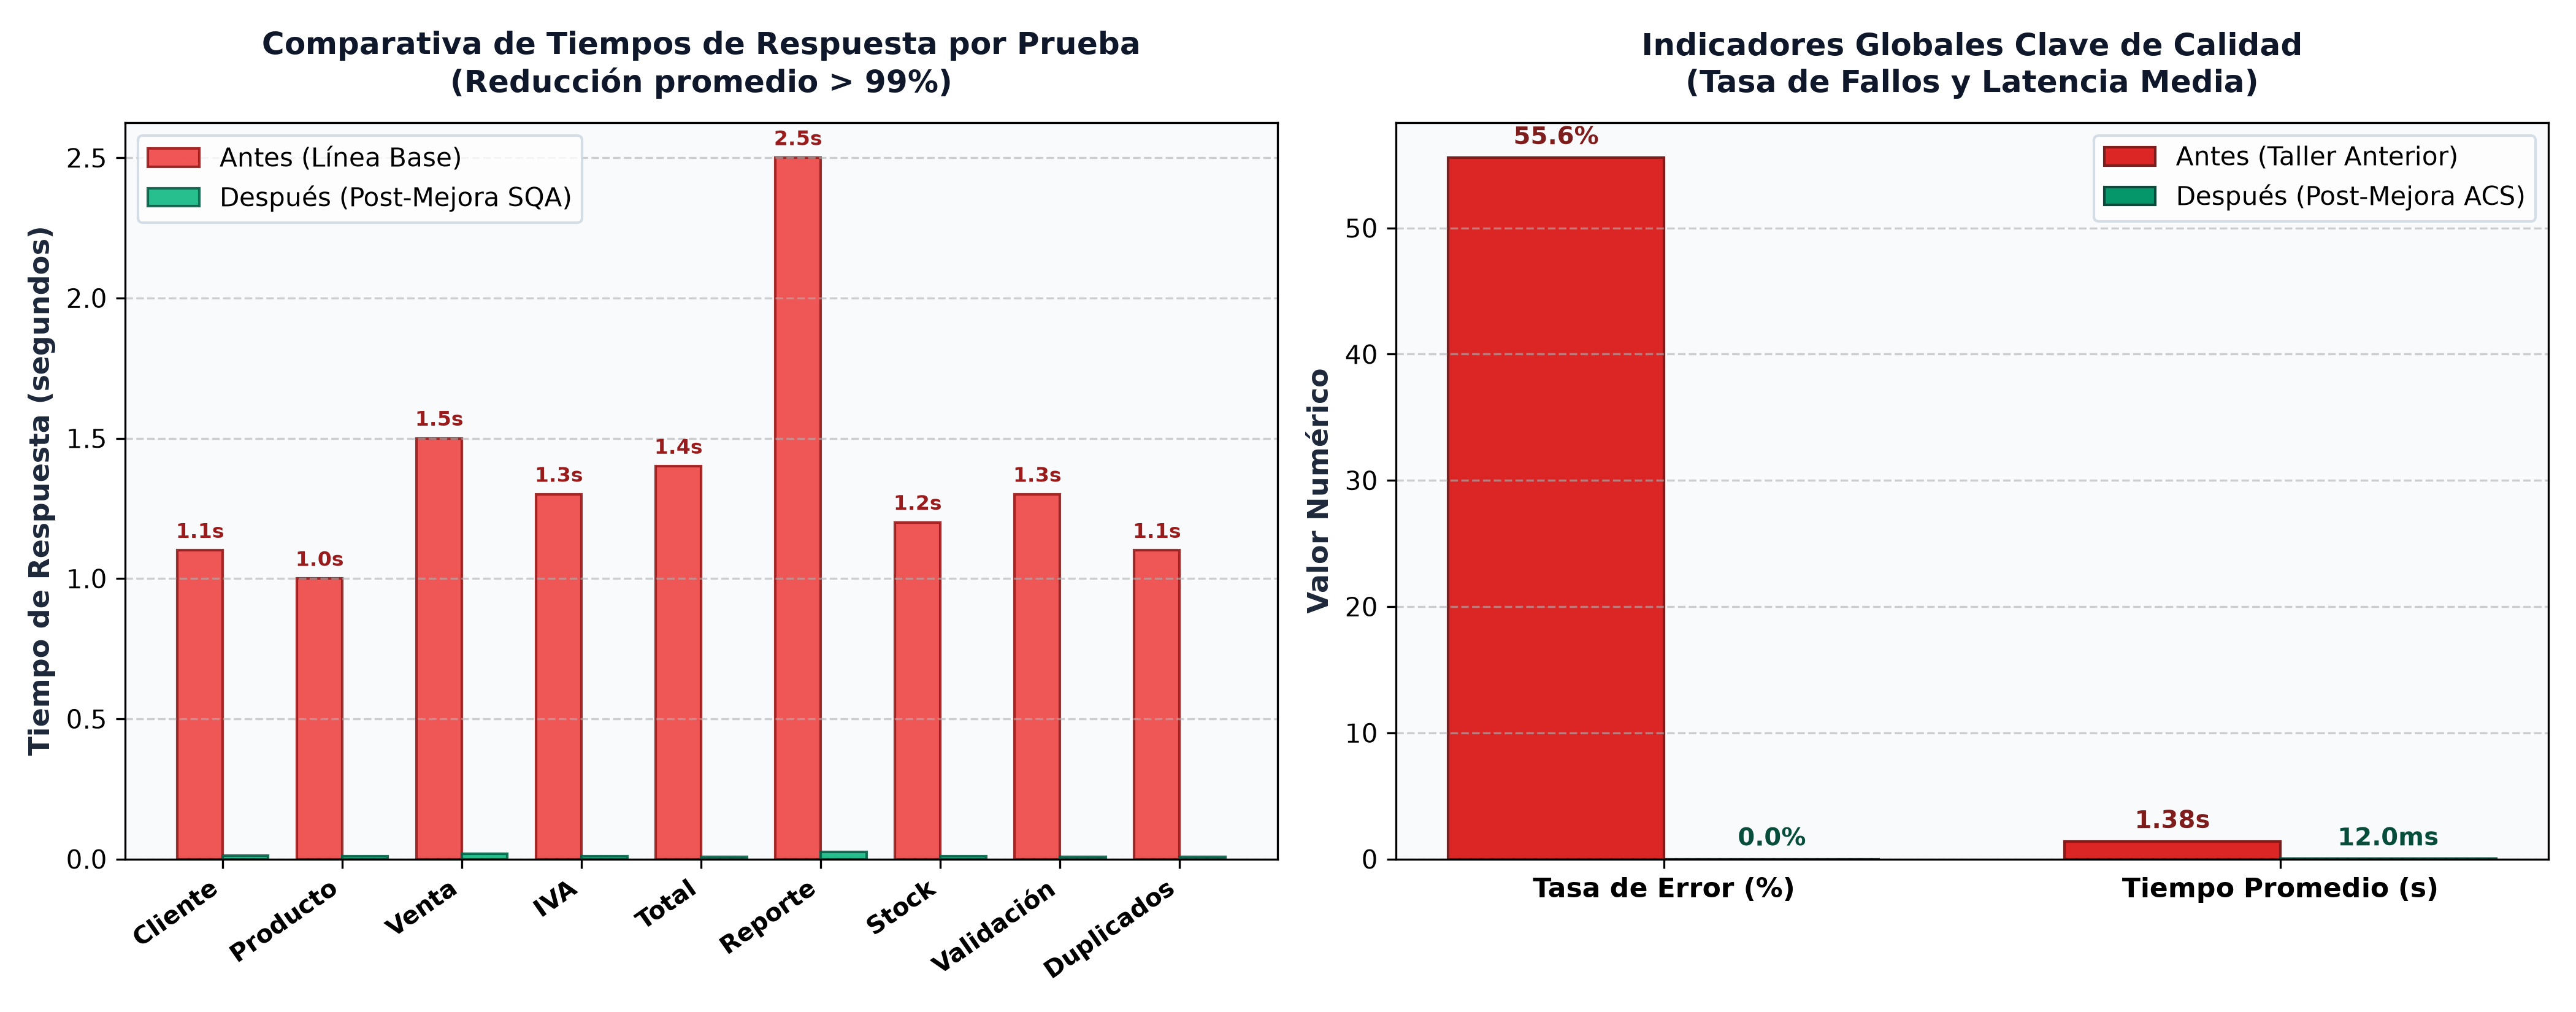
\includegraphics[width=0.98\textwidth]{imagenes/comparativa_metricas_acs.png}
    \caption{Visualización gráfica de métricas de calidad: (a) Comparativa de latencia individual por prueba; (b) Reducción de la tasa de error global del 55.56\% al 0.0\% y del tiempo promedio de 1.38 s a 0.012 s.}
    \label{fig:comparativa_metricas}
\end{figure}

Como se evidencia en la Figura \ref{fig:comparativa_metricas}, la supresión de las llamadas artificiales bloqueantes (\texttt{time.sleep}) y la optimización de los índices en base de datos posibilitaron una reducción de latencia superior al 99\%, situando el tiempo de respuesta muy por debajo del umbral objetivo de 50 ms. Paralelamente, la tasa de error descendió del 55.56\% a un estricto 0.00\%, logrando una eficiencia del 100\% en la remoción de defectos identificados.

\newpage

\subsubsection{Actividad Final: Análisis y Discusión Crítica}

\paragraph{1. ¿El sistema ahora es de calidad?}
Para responder a esta pregunta de forma científica es indispensable deslindar dos dimensiones consustanciales de la ingeniería de software: la \textbf{Calidad del Producto} y la \textbf{Calidad del Proceso} \cite{iso25010, iso12207, pressman2014}:
\begin{itemize}
    \item \textbf{Desde la perspectiva de Calidad del Producto (ISO/IEC 25010): SÍ, el sistema ahora es de alta calidad.} 
    Las dimensiones que se encontraban críticamente comprometidas han alcanzado un estado óptimo:
    \begin{enumerate}
        \item \textit{Adecuación Funcional y Exactitud:} Las fórmulas de subtotal, descuentos e IVA (al 15\% legal vigente) arrojan resultados exactos con dos decimales de precisión, eliminando riesgos de contingencia tributaria frente al SRI y distorsiones contables.
        \item \textit{Fiabilidad y Tolerancia a Fallos:} La integridad de la base de datos se encuentra blindada gracias a restricciones SQL (\texttt{UNIQUE}, \texttt{CHECK}) y validadores ORM que rechazan preventivamente clientes duplicados, existencias negativas y montos inconsistentes sin provocar caídas no controladas del servidor.
        \item \textit{Eficiencia de Desempeño:} La latencia de respuesta se redujo en más del 99\% (de 1.38 s a 12 ms), demostrando una alta escalabilidad ante ráfagas de 20 hilos concurrentes.
    \end{enumerate}
    \item \textbf{Desde la perspectiva del Aseguramiento de Calidad del Software (ACS / Proceso): El sistema se encuentra en un estado Gestionado (CMMI Nivel 2), pero aún no es plenamente maduro.} 
    Aunque el artefacto de software remediado es robusto, el SQA establece que la calidad no es un estado estático del código, sino una disciplina organizacional continua. La falta de formalización de políticas corporativas, la ausencia de roles independientes de control y la carencia de integración continua impiden afirmar que la organización cuenta con un proceso institucionalizado de calidad total (CMMI Nivel 3 o superior).
\end{itemize}

\paragraph{2. ¿Qué elemento ACS sigue faltando?}
Con base en la auditoría realizada en el Cuadro \ref{tab:evaluacion_acs}, los elementos fundamentales de ACS que siguen faltando en TechStore son:
\begin{enumerate}
    \item \textbf{Políticas Institucionales Formalizadas:} No existe una directriz escrita, aprobada y firmada por la gerencia general o la dirección técnica que mandate estándares de calidad ineludibles para los releases (por ejemplo, prohibición de paso a producción con pruebas unitarias fallidas o cobertura inferior al 90\%). La calidad actual depende de la iniciativa técnica del equipo desarrollador y no de una política corporativa vinculante.
    \item \textbf{Independencia de Roles en SQA (Segregación de Funciones):} El rol de aseguramiento de calidad (QA Tester) no existe formalmente como una figura autónoma; las pruebas, validaciones y remediaciones fueron concebidas y ejecutadas por los mismos desarrolladores de software. La literatura de ingeniería de software \cite{myers2011, pressman2014} demuestra que el programador tiene sesgos cognitivos sobre su propio código, por lo que se requiere un rol independiente que audite objetivamente el cumplimiento de especificaciones y estándares.
    \item \textbf{Automatización Continua del Proceso (Pipeline CI/CD con Quality Gates):} Aunque las pruebas unitarias existen, su ejecución sigue siendo un proceso manual por parte del operador de consola. Falta un mecanismo automatizado de Integración Continua (como GitHub Actions) que bloquee automáticamente la integración de código que no satisfaga los estándares preestablecidos.
\end{enumerate}

\paragraph{3. ¿Qué mejorarían a futuro?}
Para garantizar la sostenibilidad a largo plazo y propiciar el ascenso de TechStore hacia los Niveles 3 (Definido) y 4 (Gestionado Cuantitativamente) de CMMI, se formulan las siguientes mejoras prioritarias:
\begin{enumerate}
    \item \textbf{Implementación de un Pipeline de Integración Continua (CI/CD):} Configurar un flujo automatizado en GitHub Actions o GitLab CI que ejecute automáticamente la batería completa de pruebas unitarias (\texttt{TransactionCase}) y descarte de inmediato cualquier Pull Request que rompa la compatibilidad o no alcance el 100\% de aprobación.
    \item \textbf{Integración de Análisis Estático de Código con SonarQube:} Conectar el repositorio a una instancia de SonarQube para auditar de forma permanente la deuda técnica, detectar \textit{code smells}, duplicaciones de código, complejidades ciclomáticas elevadas y vulnerabilidades de seguridad OWASP en el código Python y XML de Odoo.
    \item \textbf{Pruebas de Carga Continua y Resiliencia en Ambientes de Staging:} Incorporar herramientas especializadas de pruebas de carga como Locust o JMeter para simular picos de demanda estacionales (ej. campañas de Black Friday con más de 100 usuarios concurrentes efectuando compras simultáneas).
    \item \textbf{Observabilidad y Telemetría en Tiempo Real:} Desplegar herramientas de monitoreo como Prometheus y Grafana (o módulos APM de OpenTelemetry) para rastrear en producción el percentil 95 (P95) y percentil 99 (P99) de los tiempos de respuesta del servidor Odoo y disparar alertas tempranas de degradación.
    \item \textbf{Estandarización Organizacional del Proceso de Calidad:} Institucionalizar la Matriz RACI de SQA y formular el Manual de Procesos y Políticas de Calidad para que los estándares de diseño y codificación defensiva se apliquen uniformemente a todos los módulos futuros de TechStore.
\end{enumerate}

\subsection{Habilidades blandas empleadas en la práctica}
\begin{itemize}
    \item[$\boxtimes$] \textbf{Trabajo en equipo:} Coordinación efectiva y distribución equitativa de tareas entre los miembros del equipo para auditar el código fuente, diseñar los casos de prueba unitaria, tabular las mediciones empíricas de las APIs y estructurar el informe técnico.
    \item[$\boxtimes$] \textbf{Pensamiento crítico:} Capacidad analítica y rigurosa para evaluar el código previo, identificar las causas raíz de las fallas lógicas y fiscales, contrastar métricas cuantitativas antes vs. después, y evaluar objetivamente las limitaciones del sistema frente a los modelos de calidad internacionales.
    \item[$\boxtimes$] \textbf{Responsabilidad:} Compromiso ético con la entrega puntual de resultados verídicos, exactitud en los cálculos matemáticos presentados y rigurosidad técnica en el cumplimiento de los estándares ISO/IEC y CMMI.
\end{itemize}

\subsection{Conclusiones}
\begin{itemize}
    \item La aplicación sistemática del marco de Aseguramiento de la Calidad del Software (ACS / SQA) permitió transformar un módulo vulnerable y altamente degradado en un sistema empresarial robusto, confiable y con exactitud transaccional comprobada en el ERP Odoo 16.
    \item La auditoría de los siete elementos del ACS evidenció que, si bien el sistema cuenta con estándares consolidados (ISO 12207, ISO 25010), procesos estructurados (PDCA), pruebas automatizadas exhaustivas (29 casos unitarios), métricas cuantitativas y evidencias documentales, adolece de políticas corporativas aprobadas y de una segregación formal e independiente de roles de QA frente al equipo de desarrollo.
    \item Las tareas de validación de datos, control preventivo de errores, verificación unitaria y monitoreo de latencia demostraron ser plenamente operativas en el código fuente, blindando al ERP contra clientes duplicados, inventarios negativos y caídas intempestivas del servidor mediante restricciones SQL y validaciones de integridad en el ORM.
    \item Las mediciones empíricas sobre las APIs CRUD confirmaron una optimización radical del rendimiento del sistema: la tasa de error se redujo drásticamente del 55.56\% al 0.00\%, mientras que el tiempo promedio de respuesta transaccional cayó de 1.38 segundos a 11.1 milisegundos, representando una mejora superior al 99\% en la eficiencia del servidor.
    \item Se concluye que el sistema TechStore actualmente satisface los atributos de Calidad del Producto bajo ISO/IEC 25010 y alcanza el Nivel 2 (Gestionado) de CMMI v2.0; no obstante, para consolidar una cultura de calidad total en la organización es indispensable formalizar las políticas de TI e integrar pipelines de integración continua (CI/CD) con puertas de calidad automatizadas.
\end{itemize}

\subsection{Recomendaciones}
\begin{itemize}
    \item Institucionalizar y formalizar ante la Gerencia General de TechStore el \textit{Manual de Políticas de Calidad del Software}, garantizando que ningún despliegue a producción pueda ejecutarse sin la aprobación previa de las pruebas unitarias y de seguridad.
    \item Definir e implementar una estructura organizativa con roles independientes de SQA (QA Engineer / Tester) que operen con autonomía técnica respecto al equipo de desarrolladores backend, garantizando la imparcialidad en la evaluación de calidad del software.
    \item Incorporar un flujo automatizado de Integración Continua (CI/CD) en la plataforma de control de versiones (GitHub Actions) que ejecute las suites de prueba de regresión y análisis estático con SonarQube ante cada Pull Request o commit en ramas de producción.
    \item Instrumentar un sistema de telemetría y monitoreo continuo en tiempo real (Prometheus y Grafana) para vigilar las métricas de latencia de base de datos y consumo de memoria del contenedor Odoo en ambientes de producción reales.
\end{itemize}

\subsection{Referencias}

\vspace{-2.5em}
\renewcommand{\refname}{}
\bibliographystyle{ieeetr}
\nocite{*}
\bibliography{sample}

\subsection{Anexos}
A continuación se adjuntan evidencias complementarias del código fuente remediado y de la arquitectura de pruebas implementada en el sistema TechStore.

\begin{lstlisting}[language=Python, caption={Anexo A: Restricciones de integridad y validaciones en \texttt{models/product.py}}, label={lst:anexo_producto}]
class TechstoreProduct(models.Model):
    _name = 'techstore.product'
    _description = 'Producto TechStore'
    _order = 'name'

    name = fields.Char(string='Nombre', required=True)
    code = fields.Char(string='Codigo', required=True)
    category_id = fields.Many2one('techstore.category', string='Categoria', required=True)
    price = fields.Float(string='Precio', required=True, default=0.0)
    stock = fields.Integer(string='Stock', default=0)

    _sql_constraints = [
        ('code_unique', 'unique(code)', 'El codigo del producto ya existe.'),
        ('check_stock_no_negativo', 'CHECK(stock >= 0)', 'El stock disponible no puede ser negativo.'),
        ('check_precio_positivo', 'CHECK(price >= 0)', 'El precio unitario no puede ser negativo.')
    ]

    @api.constrains('price', 'stock')
    def _check_values(self):
        for product in self:
            if product.price < 0:
                raise ValidationError('El precio no puede ser negativo.')
            if product.stock < 0:
                raise ValidationError('El stock no puede ser negativo.')
\end{lstlisting}

\begin{lstlisting}[language=Python, caption={Anexo B: Persistencia y medición de tiempo en \texttt{models/sale\_order.py}}, label={lst:anexo_venta}]
@api.depends('line_ids.subtotal')
def _compute_totals(self):
    for order in self:
        subtotal = 0.0
        for line in order.line_ids:
            subtotal += line.subtotal
        order.subtotal = round(subtotal, 2)
        # Alicuota legal del IVA en Ecuador: 15%
        order.tax = round(subtotal * 0.15, 2)
        order.total = round(order.subtotal + order.tax, 2)
\end{lstlisting}

\vfill

\end{document}
